\RequirePackage{etex}
\RequirePackage{fix-cm} % For custom font shaping


% Document class
\documentclass[pdftex, 11pt, a4paper, oneside, english]{memoir}



% Page styling
\let\footruleskip\undefined
\usepackage{fancyhdr}
\pagestyle{fancy}

% English language package
\usepackage[english]{babel}

% UTF-8 characters
\usepackage[utf8]{inputenc}

% Package for dummy text
\usepackage{lipsum}

% Colors for chapters and table of content
\usepackage[table,xcdraw]{xcolor}
\definecolor{ThemeColor}{RGB}{51, 102, 255} % Blue
\definecolor{BlackColor}{RGB}{0, 0, 0} % Black

\usepackage{pdfpages}

% Table packages
% Merge cells i tables
\usepackage{multirow}
\usepackage{makecell}
\usepackage{tabularx}

% PDF propeties (fx. hyperlinks, pdftitle)
\usepackage[hyphens]{url}
\usepackage[bookmarks=true,bookmarksnumbered=true,citecolor=black,colorlinks=true,hyperfigures=true,hyperfootnotes=true,hyperindex=true,linkcolor=black,urlcolor=blue]{hyperref}

% BibTeX = bibliography
% ALWAYS USE \citep{} or something like:
% \citep[see this baws article]{fooArticle}
\usepackage[semicolon,authoryear,round]{natbib}
\bibliographystyle{plainnat}

% Package for editing captions. Fx for figures and code listings
\usepackage[textfont={footnotesize,sl}]{caption}

%Package for MATLAB code
\usepackage[framed, numbered]{mcode}

% Package for more elegant math
\usepackage{amsmath}
\usepackage{xfrac} % for \sfrac command


% Styles
% Package for setup of chapters and sections
\usepackage{titlesec}


% % % % % % % % % % % % % % CHAPTER  % % % % % % % % % % % % % % % % % % % % % %
% Define fontsize for the numbering of the chapters
\newcommand{\ChapterNumbering}{
    \usefont{\encodingdefault}{\rmdefault}{b}{n}
    \fontsize{35}{45}\normalfont\color{ThemeColor}}

% Chapter numbers in margin
\chapterstyle{hangnum}

% Modifying "\chapterstyle{hangnum}"
% Changing vertical position of chapter headline
\renewcommand*{\chapterheadstart}{\vspace*{-20pt}}

% Color setup for chapters
% Title color
\renewcommand*{\chaptitlefont}{\bfseries\Huge\color{BlackColor}}
% Number color
\renewcommand{\chapnumfont}{\normalfont\ChapterNumbering\color{ThemeColor}}




% % % % % % % % % % % % % % SECTION  % % % % % % % % % % % % % % % % % % % % % %
% Section numbers in margin
\hangsecnum

% Color setup for sections
% Title color
%\renewcommand\thesection{\color{ThemeColor}\thechapter.\arabic{section}}
\renewcommand\thesection{\thechapter.\arabic{section}}

% Set numbering depth of sections
\setsecnumdepth{subsubsection}

% Set the depth of sections included in table of contents
\settocdepth{subsection}



% Clear all header an footer fields
\fancyhf{}


% % % % % % % % % % % % % % HEADER % % % % % % % % % % % % % % % % % % % % % % %
% Delete headruler
\renewcommand{\headrulewidth}{0pt}

% Insert picture in left side on even pages and right side on odd pages
%\fancyhead[R]{
\includegraphics[height=40pt]{figure/header/header}}



% % % % % % % % % % % % % % FOOTER % % % % % % % % % % % % % % % % % % % % % % %
% Insert pagenumber on right side of even page, left side of odd page
\fancyfoot[R]{\thepage}

\setlength\headheight{44.1pt}

%\setcounter{page}{1}

%%%%%%%%%%%%%%%%%%%%%%%%%%%%%%%%%%%%%%%%%%%%%%%%%%%%%%%%%%%%%%%%%%%%%%%%%%%%%%%%
%                       Custom for figures (myFigure etc.)                     %
%                     			      	        		                       %
%%%%%%%%%%%%%%%%%%%%%%%%%%%%%%%%%%%%%%%%%%%%%%%%%%%%%%%%%%%%%%%%%%%%%%%%%%%%%%%%

% Include image and graphic
\usepackage{graphicx}

% Package for wrapping figures in text
\usepackage{wrapfig}

% Set the path where LaTeX looks for pictures.
\graphicspath{{figure/}}

% You need a newsubfloat element to use subcaption
\newsubfloat{figure}

% Command to set caption styles
\captionsetup[figure]{
    labelfont=bf
}

\captionsetup[table]{
    labelfont=bf
}

% from the old preamble
\captionnamefont{\bfseries\small}
\captiontitlefont{\itshape\small}
\subcaptionlabelfont{\bfseries\small}
\subcaptionfont{\itshape\small}


% Command \myFigure{filename}{caption}{label}{width} 
% for inserting a new figure.
\newcommand{\myFigure}[4]
{ 
    \begin{figure}[ht] 
        \centering 
        \includegraphics[width=#4\textwidth]{#1} 
        \caption{#2} 
        \label{#3} 
    \end{figure}
} 

\newcommand{\myFigureWithRotation}[5]
{ 
	\begin{figure}[ht] 
		\centering 
		\includegraphics[width=#4\textwidth, angle=#5]{#1} 
		\caption{#2} 
		\label{#3} 
	\end{figure}
} 
 
% Insert a figure wraped in text (left/right)
% Command \myWrapFigure{filename}{caption}{label}{width}{r/l}
\newcommand{\myWrapFigure}[5]
{ 
    \begin{wrapfigure}{#5}{#4 \textwidth}
        \begin{center}
            \includegraphics[width=#4\textwidth]{#1}
        \end{center}
        \caption{#2}
        \label{#3} 
    \end{wrapfigure}
}
 
% Insert two figures side by side, with a caption covering both and a subcaption for each figure. OBS: scaled for 50 % text width both
% Command \mySubFigure{filename1}{filename2}{caption}
% {subcaption1}{subcaption2}{label}{sublabel1}{sublabel2}
\newcommand{\mySubFigure}[9]
{
    \begin{figure}[ht]
        \centering
        \subbottom[{#4}\label{#7}]%
            {\includegraphics[width=0.47\textwidth]{#1}}\hfill
        \subbottom[{#5}\label{#8}]%
            {\includegraphics[width=0.47\textwidth]{#2}}
        \caption{#3}
        \label{#6}
    \end{figure}
}


% Keeps floats in the section. 
% Help control place to put pix
\usepackage[section]{placeins}


%Package with enumirate command with extra options (used within cells of tabular)
\usepackage[inline]{enumitem}
\usepackage[]{todonotes}


% new commands for individually colored todo 
\newcommand{\todorene}[2]{
\todo[#1, color=green!40]{#2 \\- Rene}
}

\usepackage[utf8]{inputenc}

% Default fixed font does not support bold face
\DeclareFixedFont{\ttb}{T1}{txtt}{bx}{n}{8} % for bold
\DeclareFixedFont{\ttm}{T1}{txtt}{m}{n}{8}  % for normal


\definecolor{deepblue}{rgb}{0,0,0.5}
\definecolor{deepred}{rgb}{0.6,0,0}
\definecolor{deepgreen}{rgb}{0,0.5,0}

\usepackage{listings}

% Python style for highlighting
\newcommand\pythonstyle{\lstset{

}}


%New colors defined below
\definecolor{codegreen}{rgb}{0,0.6,0}
\definecolor{codegray}{rgb}{0.5,0.5,0.5}
\definecolor{codepurple}{rgb}{0.58,0,0.82}
\definecolor{backcolour}{rgb}{0.95,0.95,0.92}

%Code listing style named "mystyle"
\lstdefinestyle{python}{
	%keepspaces=true,
	language=python,
	showtabs=true,
	tab=,
	tabsize=2,
	basicstyle=\ttfamily\footnotesize,%\setstretch{.5},
	stringstyle=\color{stringcolour},
	showstringspaces=false,
	alsoletter={1234567890},
	otherkeywords={\%, \}, \{, \&, \|},
	keywordstyle=\color{keywordcolour}\bfseries,
	emph={and,break,class,continue,def,yield,del,elif ,else,%
		except,exec,finally,for,from,global,if,import,in,%
		lambda,not,or,pass,print,raise,return,try,while,assert,with},
	emphstyle=\color{blue}\bfseries,
	emph={[2]True, False, None},
	emphstyle=[2]\color{keywordcolour},
	emph={[3]object,type,isinstance,copy,deepcopy,zip,enumerate,reversed,list,set,len,dict,tuple,xrange,append,execfile,real,imag,reduce,str,repr},
	emphstyle=[3]\color{commandcolour},
	emph={Exception,NameError,IndexError,SyntaxError,TypeError,ValueError,OverflowError,ZeroDivisionError},
	emphstyle=\color{exceptioncolour}\bfseries,
	%upquote=true,
	morecomment=[s]{"""}{"""},
	commentstyle=\color{commentcolour}\slshape,
	%emph={[4]1, 2, 3, 4, 5, 6, 7, 8, 9, 0},
	emph={[4]ode, fsolve, sqrt, exp, sin, cos,arctan, arctan2, arccos, pi,  array, norm, solve, dot, arange, isscalar, max, sum, flatten, shape, reshape, find, any, all, abs, plot, linspace, legend, quad, polyval,polyfit, hstack, concatenate,vstack,column_stack,empty,zeros,ones,rand,vander,grid,pcolor,eig,eigs,eigvals,svd,qr,tan,det,logspace,roll,min,mean,cumsum,cumprod,diff,vectorize,lstsq,cla,eye,xlabel,ylabel,squeeze},
	emphstyle=[4]\color{numpycolour},
	emph={[5]__init__,__add__,__mul__,__div__,__sub__,__call__,__getitem__,__setitem__,__eq__,__ne__,__nonzero__,__rmul__,__radd__,__repr__,__str__,__get__,__truediv__,__pow__,__name__,__future__,__all__},
	emphstyle=[5]\color{specmethodcolour},
	emph={[6]assert,yield},
	emphstyle=[6]\color{keywordcolour}\bfseries,
	emph={[7]range},
	emphstyle={[7]\color{keywordcolour}\bfseries},
	% emph={[7]self},
	% emphstyle=[7]\bfseries,
	literate=*%
	{:}{{\literatecolour:}}{1}%
	{=}{{\literatecolour=}}{1}%
	{-}{{\literatecolour-}}{1}%
	{+}{{\literatecolour+}}{1}%
	{*}{{\literatecolour*}}{1}%
	{**}{{\literatecolour{**}}}2%
	{/}{{\literatecolour/}}{1}%
	{//}{{\literatecolour{//}}}2%
	{!}{{\literatecolour!}}{1}%
	%{(}{{\literatecolour(}}{1}%
	%{)}{{\literatecolour)}}{1}%
	{[}{{\literatecolour[}}{1}%
	{]}{{\literatecolour]}}{1}%
	{<}{{\literatecolour<}}{1}%
	{>}{{\literatecolour>}}{1}%
	{>>>}{\pythonprompt}{3}%
	,%
	%aboveskip=.5ex,
	frame=trbl,
	%frameround=tttt,
	%framesep=.3ex,
	rulecolor=\color{black!40},
	%framexleftmargin=\framemargin,
	%framextopmargin=.1ex,
	%framexbottommargin=.1ex,
	%framexrightmargin=\framemargin,
	%framexleftmargin=1mm, framextopmargin=1mm, frame=shadowbox, rulesepcolor=\color{blue},#1
	%frame=tb,
	backgroundcolor=\color{white},
	breakindent=.5\textwidth,frame=single,breaklines=true%
	%}
}
%%%%%%%%%%%%%%%%%%%%%%%%%%%%%%%%%%%%%%%%%%%%%%%%%%%%%%%%%%%%%%%%%%%%%%%%%%%%%%%%
%                           Custom Commands                                    %
%                                                                              %
%%%%%%%%%%%%%%%%%%%%%%%%%%%%%%%%%%%%%%%%%%%%%%%%%%%%%%%%%%%%%%%%%%%%%%%%%%%%%%%%

%%%%% FIGURES %%%%%
% The following commands are defined in: style/figure

% Insert a new figure:
% \myFigure{filename}{caption}{label}{width}
% width is ratio of textwidth, so it should be between 0.1 and 1

% Insert a figure wraped in text (left/right)
% \myWrapFigure{filename}{caption}{label}{width}{l/r}
% width is ratio of textwidth, so it should be between 0.1 and 1
% l/r: l = left, r = right

% Insert two figures side by side, with a caption covering both and a subcaption for each figure. OBS: scaled for 50 % text width both
% Command \mySubFigure{filename1}{filename2}{caption}
% {subcaption1}{subcaption2}{label}{sublabel1}{sublabel2}



%%%%% TABLES %%%%%
% Command \myTable{caption text}{refrence label}{input filename: eq <tables/myTable>}
% for inserting tables


%%%%% CODE LISTING %%%%%
%\begin{lstlisting}[language=Matlab, caption={Dette er et eksempel på hvordan du skal bruge listing}, label=list_me_like_a_baws]
%
%	INSERT CODE HERE
%
%\end{lstlisting}

% For more info go to http://ctan.org/pkg/listing



%%%%% EQUATIONS / MATH %%%%%
% For info in the user guide at http://ctan.org/pkg/amsmath
% Feel free to add ninja tricks to this guide



%%%%% BibTeX %%%%%
% To cite some article use:
% \citep{fooArticle} or
% \citep[see this baws article]{fooArticle}

% OBS: remember to add article to "bibliografi.bib" using syntex of the examples in the file.



%%%%% Nomenclature %%%%%
% When introducing a new symbol add it to the nomenclature by:
% \nomenclature{symbol}{description}
% remember to put symbol in mathmode if necessary
% OBS: if you need to add more the one symbol you have to add a "%" at the end of every \nomenclature use except for the last one. See example below:
%
%	\begin{equation}
%		e=m \cdot c^2
%	\end{equation}%
%	\nomenclature{$e$}{Energy}%
%	\nomenclature{$m$}{The mass}%
%	\nomenclature{$c$}{The speed of light. 299 792 458 $\frac{m}{s}$}

%%%%% COLOR %%%%%
\definecolor{deadlinecolor}{HTML}{FD6864}
\definecolor{reviewcolor}{HTML}{9698ED}

%%%%% TEXT COMMANDS %%%%%
\newcommand{\prbl}{Problematic} % For the lulz

%%%%% MATH COMMANDS %%%%%
\newcommand{\degree}{^\circ}

% Command \myTable{caption text}{refrence label}{input filename: eq <tables/myTable>}
% for inserting tables
\newcommand{\myTable}[3]
{ 
    \begin{table}[h]
    \centering
    \caption{#1}
    \label{#2}
        \input{#3}
    \end{table}
}
% Example on content in table file
%
%    \begin{tabular}{rll}
%    \multicolumn{1}{c}{\textbf{Tapsstørrelse}} &
%    \multicolumn{1}{c}{\textbf{Målt beregningstid}} \\ \hline
%       1      &  35,6  $\mu s$     \\[0.05cm] 
%       2      &  36,5  $\mu s$     \\[0.05cm] 
%       5      &  32,0  $\mu s$     \\[0.05cm] 
%       8      &  32,0  $\mu s$     \\[0.05cm] 
%       10     &  32,0  $\mu s$     \\[0.05cm] 
%       20     &  32,5  $\mu s$     \\[0.05cm] 
%       50     &  69,0  $\mu s$     \\[0.05cm] 
%       80     &  101,5 $\mu s$     \\[0.05cm] 
%       100    &  124,5 $\mu s$     \\[0.05cm] 
%       200    &  240,5 $\mu s$     \\[0.05cm] 
%       500    &  587   $\mu s$     \\[0.05cm] 
%       800    &  932   $\mu s$     \\[0.05cm] 
%       1000   &  1164  $\mu s$     \\[0.05cm] 
%       1024   &  1192  $\mu s$     \\[0.05cm]
%       \hline
%       512    &  601   $\mu s$     \\[0.05cm]
%       513    &  605   $\mu s$     \\
%    \end{tabular}



% Geometry for frontpage
\usepackage{geometry}

% For traceability matrix
\usepackage{longtable}
\usepackage{rotating}

\usepackage{subcaption}
\usepackage{tabularx}

\begin{document}

	\begin{titlingpage}
		% Frontpage goes here
		\newgeometry{left=3cm,bottom=0.1cm}

\centerline{\Huge\bfseries\color{ThemeColor} Deep learning}

\vspace{5em}
\centerline{\large\bfseries\color{BlackColor}}
\vspace{0.5em}
\centerline{\large\color{BlackColor}Department of Engineering - Aarhus University}

\vspace{0.5em}
\centerline{\large\color{BlackColor} June 15, 2017}
\vspace{0.5em}
\centerline{\large\color{BlackColor} Group 3}



\vspace{25em}

\begin{center}
	\centerline{\large\color{BlackColor} }
	\vspace{5em}
   \begin{tabular}{ l p{3cm} l l }
    Stud. no.: 201270762 && René Rotvig Jensen & \\\hline
	& & \\
	Stud. no.: 201270868 && Peter Kragelund & \\\hline
	& & \\
	Stud. no.: 09641 && Troels Thomsen & \\\hline
   \end{tabular}
\end{center}
\thispagestyle{empty} % No header and footer on this page
\restoregeometry


	\end{titlingpage}
	
    % Table of contents
    \tableofcontents*	% The star keeps TOC from indexing itself

    \chapter{Introduction}
\label{chp:intro}


    \chapter{Theory}
\label{chp:theory}

\section{RegularNet}
\section{Deep Residual Networks - ResNet}
\section{Densely Connected Convolutional Networks - DenseNet}
    \chapter{Implementation}
\label{chp:impl}
\section{Feature Invariance}
\section{Deep Neural Net - RegularNet}
%composed exclusively of regular and strided convolutional layers. While this architecture works well for relatively shallow networks, it becomes increasingly more difficult to train as the network depth increases.
\section{Deep Residual Networks - ResNet}
\section{Densely Connected Convolutional Networks - DenseNet}
    \chapter{Results}
\label{chp:results}

\section{Test Method}

This section will describe the test methods used to test the different models. The test methods will produce a set of results for each model, which will be compared in the discussion chapter.

\begin{lstlisting}[language=Python, label=lst:CalcAcc, caption=Function to calculate the test accuracy for a model]
# Calculate test accuracy
def CalcTestAccuracy(sess, data, labels, isTransformed):
    
    percentageList = np.zeros(10)
    
    yT = np.reshape(np.array(labels),[len(labels)])
    if(isTransformed):
        lossT,yP = sess.run([loss,output],
        	feed_dict={input_layer:data.eval(),label_layer:yT})
    else:
        lossT,yP = sess.run([loss,output],
        	feed_dict={input_layer:data,label_layer:yT})
    
    equal = np.equal(yT,np.argmax(yP,1))
    accuracy = np.sum(equal)/float(len(yT))
    print "Test set accuracy: " + str(accuracy)
    
    for i in range(0,len(yT)):
        if equal[i] == False:
            index = yT[i]
            percentageList[index] += 1
    
    return accuracy, percentageList
\end{lstlisting}

Listing \ref{lst:CalcAcc} shows the code for calculating the test accuracy for a model. A Tensorflow session is passed to the function, which makes it possible to run the session, and collect the classifications for the passed data. The classification from the model is checked against the true label, and if the model classified correctly, true will be returned. If the model classified wrong, false will be returned. To calculate the accuray the sum of all the correct classifications is divided with the total amount of data samples. For each wrong classification the percentageList counts one up on the index for the label of the wrong classification. Meaning that if an airplane (0) was wrongly classified, the percentageList would be counted one up at index 0. This is in the RotateAndCalc function used to calculate the failure percentage belonging to each label.

The testing is seperated into scramble classification and label wise classification. Scramble classification is where the data used is selected across all the labels, where label wise is where the data used for classification is only for one specific label at a time.

\begin{lstlisting}[language=Python, label=lst:testing, caption=Testing the classification abilities for the model]
with tf.Session() as sess:
    saver.restore(sess, "./trainingmodels/DenseNet/model_densenet.ckpt")
    print "Model restored."
    
    numbOfImg = 1000 #Number of images to be found
    finalLabelList = [] #List with each labellist inside it
    
    #Scramble classification
    print "Scramble classification"
    sImages, sLabels = GetScrambleData(2000)
    sAcc, sPrc = RotateAndCalc(sess, sImages, sLabels)
    print "Percentage for failing classification: "
    print sPrc
    print "Total accuracy for the test set: " + str(sAcc[0])
    PlotAcc(sAcc)
    
    #Label wise classification
    print "Label wise classification"
    for label in range(0,10): #Label value 0-9
        print "Classifying on label: " + str(label)
        images, labels = GetLabelData(numbOfImg)
        lAcc,_ = RotateAndCalc(sess, images, labels)
        finalLabelList.append(lAcc)
        PlotAcc(lAcc)
    
    # Print all the label wise in same plot
    Labels = ['Airplane', 'Automobile', 'Bird', 'Cat', 'Deer', 'Dog', 
    		'Frog', 'Horse', 'Ship', 'Truck']
    for i in range(len(finalLabelList)):
        x = np.arange(0, 360, 10)
        plt.xlabel('Degree')
        plt.ylabel('Accuracy')
        plt.title('Accuracy with rotating images')
        plt.plot(x,finalLabelList[i], label=Labels[i])

    plt.legend(bbox_to_anchor=(1.05, 1), loc=2, borderaxespad=0.)
    plt.show()
\end{lstlisting}

Listing \ref{lst:testing} show the scramble and label wise classification testing. In scramble classification 2000 samples of data is rotated from 0 to 350 degree, while the accuracy for these rotated images is calculated. A mean percentage for the failing classifications is printed alongside a plot of the accurcay from 0 to 350 degree rotations. The label wise classification run through all 10 labels (label 0 to 9), and collects and rotate images for the specific label. The accuracy for each rotated label classification is plotted. At last all the accuracy plots for all labels are plotted on one plot.

\section{Scrambled Classification - Reading Guide}
A scrambled classification has been performed. The test set consist of 2000 label wise mixed images. The images has been obtained from the Cifar-10 test batch.
All figures has \emph{Accuracy} on the y-axis which is the mean of all the accuracies and \emph{Degree} on the x-axis - degrees represent the amount the image has been rotated. 0 degrees is the original position. A sample has been taking for each 10 degree the image has been rotated.

The tables has been created by taking the total amount of falsely classified images, and then it has been separated into the separate labels and the percentage which is shown represent the amount of falsely classified label.

\section{Label wise Classification - Reading Guide}
A label wise classification has been performed on 500 images from the Cifar-10 test batch. All the results for the separate labels can be seen in the following subsections. At the end a label wise collective plot consisting of all the separate labels in one plot has been created for comparison.
All figures has \emph{Accuracy} on the y-axis which is the mean of all the accuracies and \emph{Degree} on the x-axis - degrees represent the amount the image has been rotated. 0 degrees is the original position. A sample has been taking for each 10 degree the image has been rotated.

\section{Deep Neural Net - RegularNet}
This section is for all the results of the Regular neural net.
\subsection{Scrambled Classification}
\myFigure{results/RegularNet/scrambled/scrambled2000.PNG}{2000 images with rotation from 0 - 360 degrees (RegularNet)}{fig:scramReg}{0.8}
\FloatBarrier

\begin{table}[]
	\centering
	\caption{Percentage of falsely classified images separated into labels (RegularNet)}
	\label{table:falseclasReg}
	\begin{tabular}{llllllllll}
		Airplane & Automobile & Bird     & Cat    & Deer     & Dog     & Frog   & Horse    & Ship         & Truck         \\
		8.58 \%  & 8.93 \%    & 11.197 \% & 10.75 \% & 9.6 \% & 8.43 \% & 7.8 \% & 11.22 \% & 12.17 \% & 11.32 \%
	\end{tabular}
\end{table}
\FloatBarrier
\subsection{Label wise Classification}
\subsubsection{Label 0 - Airplane}
\myFigure{results/RegularNet/LabelWise/label0_500.PNG}{Label 0 - Airplane (RegularNet)}{fig:airplane}{0.8}
\FloatBarrier
\subsubsection{Label 1 - Automobile}
\myFigure{results/RegularNet/LabelWise/label1_500.PNG}{Label 1 - Automobile (RegularNet)}{fig:automobile}{0.8}
\FloatBarrier
\subsubsection{Label 2 - Bird}
\myFigure{results/RegularNet/LabelWise/label2_500.PNG}{Label 2 - Bird (RegularNet)}{fig:bird}{0.8}
\FloatBarrier
\subsubsection{Label 3 - Cat}
\myFigure{results/RegularNet/LabelWise/label3_500.PNG}{Label 3 - Cat (RegularNet)}{fig:cat}{0.8}
\FloatBarrier
\subsubsection{Label 4 - Deer}
\myFigure{results/RegularNet/LabelWise/label4_500.PNG}{Label 4 - Deer (RegularNet)}{fig:deer}{0.8}
\FloatBarrier
\subsubsection{Label 5 - Dog}
\myFigure{results/RegularNet/LabelWise/label5_500.PNG}{Label 5 - Dog (RegularNet)}{fig:dog}{0.8}
\FloatBarrier
\subsubsection{Label 6 - Frog}
\myFigure{results/RegularNet/LabelWise/label6_500.PNG}{Label 6 - Frog (RegularNet)}{fig:intro}{0.8}
\FloatBarrier
\subsubsection{Label 7 - Horse}
\myFigure{results/RegularNet/LabelWise/label7_500.PNG}{Label 7 - Horse (RegularNet)}{fig:horse}{0.8}
\FloatBarrier
\subsubsection{Label 8 - Ship}
\myFigure{results/RegularNet/LabelWise/label8_500.PNG}{Label 0 - Ship (RegularNet)}{fig:ship}{0.8}
\FloatBarrier
\subsubsection{Label 9 - Truck}
\myFigure{results/RegularNet/LabelWise/label9_500.PNG}{Label 9 - Truck (RegularNet)}{fig:truck}{0.8}
\FloatBarrier
\subsubsection{Collective Label Wise Results}
\myFigure{results/RegularNet/LabelWise/all_500.PNG}{Collective label wise results (RegularNet)}{fig:colReg}{1}
\FloatBarrier

\section{Deep Residual Networks - ResNet}
This section is for all the results of the Deep residual network.
\subsection{Scrambled Classification}
\myFigure{results/ResNet/scrambled/scrambled2000.PNG}{2000 images with rotation from 0 - 360 degrees (ResNet)}{fig:scramRes}{0.8}
\FloatBarrier

\begin{table}[]
	\centering
	\caption{Percentage of falsely classified images separated into labels (ResNet)}
	\label{table:falseclasRes}
	\begin{tabular}{llllllllll}
		Airplane & Automobile & Bird     & Cat    & Deer     & Dog     & Frog   & Horse    & Ship         & Truck         \\
		9.7 \%  & 9.1 \%    & 10.17 \% & 9.8 \% & 10.1 \% & 8.4\% & 8.6 \% & 11.22 \% & 11.47 \% & 11.47 \%
	\end{tabular}
\end{table}
\FloatBarrier
\subsection{Label Wise Classification}
\subsubsection{Label 0 - Airplane}
\myFigure{results/ResNet/LabelWise/label0_500.PNG}{Label 0 - Airplane (ResNet)}{fig:airplaneRes}{0.8}
\FloatBarrier
\subsubsection{Label 1 - Automobile}
\myFigure{results/ResNet/LabelWise/label1_500.PNG}{Label 1 - Automobile (ResNet)}{fig:automobileRes}{0.8}
\FloatBarrier
\subsubsection{Label 2 - Bird}
\myFigure{results/ResNet/LabelWise/label2_500.PNG}{Label 2 - Bird (ResNet)}{fig:birdRes}{0.8}
\FloatBarrier
\subsubsection{Label 3 - Cat}
\myFigure{results/ResNet/LabelWise/label3_500.PNG}{Label 3 - Cat (ResNet)}{fig:catRes}{0.8}
\FloatBarrier
\subsubsection{Label 4 - Deer}
\myFigure{results/ResNet/LabelWise/label4_500.PNG}{Label 4 - Deer (ResNet)}{fig:deerRes}{0.8}
\FloatBarrier
\subsubsection{Label 5 - Dog}
\myFigure{results/ResNet/LabelWise/label5_500.PNG}{Label 5 - Dog (ResNet)}{fig:dogRes}{0.8}
\FloatBarrier
\subsubsection{Label 6 - Frog}
\myFigure{results/ResNet/LabelWise/label6_500.PNG}{Label 6 - Frog (ResNet)}{fig:introRes}{0.8}
\FloatBarrier
\subsubsection{Label 7 - Horse}
\myFigure{results/ResNet/LabelWise/label7_500.PNG}{Label 7 - Horse (ResNet)}{fig:horseRes}{0.8}
\FloatBarrier
\subsubsection{Label 8 - Ship}
\myFigure{results/ResNet/LabelWise/label8_500.PNG}{Label 0 - Ship (ResNet)}{fig:shipRes}{0.8}
\FloatBarrier
\subsubsection{Label 9 - Truck}
\myFigure{results/ResNet/LabelWise/label9_500.PNG}{Label 9 - Truck (ResNet)}{fig:truckRes}{0.8}
\FloatBarrier
\subsubsection{Collective Label Wise Results}
\myFigure{results/ResNet/LabelWise/all_500.PNG}{Collective label wise results (ResNet)}{fig:colRes}{1}
\FloatBarrier

\section{Densely Connected Convolutional Networks - DenseNet}
This section is for all the results of the Densely connected convolutional network.

\subsection{Scrambled Classification}

\myFigure{results/DenseNet/scrambled/scrambled2000.PNG}{2000 images with rotation from 0 - 360 degrees}{fig:scram}{0.8}
\FloatBarrier

\begin{table}[]
	\centering
	\caption{Percentage of falsely classified images separated into labels }
	\label{table:falseclas}
	\begin{tabular}{llllllllll}
		Airplane & Automobile & Bird     & Cat    & Deer     & Dog     & Frog   & Horse    & Ship         & Truck         \\
		9.71 \%  & 9.07 \%    & 10.17 \% & 9.8 \% & 10.12 \% & 8.38 \% & 8.6 \% & 11.22 \% & 11.468458 \% & 11.4684576 \%
	\end{tabular}
\end{table}
\FloatBarrier
\subsection{Label wise Classification}
\subsubsection{Label 0 - Airplane}
\myFigure{results/DenseNet/LabelWise/label0_500.PNG}{Label 0 - Airplane (DenseNet)}{fig:airplaneDense}{0.8}
\FloatBarrier
\subsubsection{Label 1 - Automobile}
\myFigure{results/DenseNet/LabelWise/label1_500.PNG}{Label 1 - Automobile (DenseNet)}{fig:automobileDense}{0.8}
\FloatBarrier
\subsubsection{Label 2 - Bird}
\myFigure{results/DenseNet/LabelWise/label2_500.PNG}{Label 2 - Bird (DenseNet)}{fig:birdDense}{0.8}
\FloatBarrier
\subsubsection{Label 3 - Cat}
\myFigure{results/DenseNet/LabelWise/label3_500.PNG}{Label 3 - Cat (DenseNet)}{fig:catDense}{0.8}
\FloatBarrier
\subsubsection{Label 4 - Deer}
\myFigure{results/DenseNet/LabelWise/label4_500.PNG}{Label 4 - Deer (DenseNet)}{fig:deerDense}{0.8}
\FloatBarrier
\subsubsection{Label 5 - Dog}
\myFigure{results/DenseNet/LabelWise/label5_500.PNG}{Label 5 - Dog (DenseNet)}{fig:dogDense}{0.8}
\FloatBarrier
\subsubsection{Label 6 - Frog}
\myFigure{results/DenseNet/LabelWise/label6_500.PNG}{Label 6 - Frog (DenseNet)}{fig:introDense}{0.8}
\FloatBarrier
\subsubsection{Label 7 - Horse}
\myFigure{results/DenseNet/LabelWise/label7_500.PNG}{Label 7 - Horse (DenseNet)}{fig:horseDense}{0.8}
\FloatBarrier
\subsubsection{Label 8 - Ship}
\myFigure{results/DenseNet/LabelWise/label8_500.PNG}{Label 0 - Ship (DenseNet)}{fig:shipDense}{0.8}
\FloatBarrier
\subsubsection{Label 9 - Truck}
\myFigure{results/DenseNet/LabelWise/label9_500.PNG}{Label 9 - Truck (DenseNet)}{fig:truckDense}{0.8}
\FloatBarrier
\subsubsection{Collective Label Wise Results}
\myFigure{results/DenseNet/LabelWise/all_500.PNG}{Collective label wise results (DenseNet)}{fig:colDense}{1}
\FloatBarrier
    \chapter{Discussion}
\label{chp:discussion}

\subsection{Implementation Experience}

The main purpose of this project was to compare the three neural networks a deep neural network, a deep residual network and a densely connected convolutional network. The different networks have different depth and different architecture. The first experience was the different time and memory required to train the models on the small images from the CIFAR-10 data set. On a nvidia geforce gtx 960 2gb Graphics Processing Unit, it took around two hours to train the RegularNet, two hours and 45 minutes to train the ResNet, while with the DenseNet it was not possible to train the model at all, due to memory shortage in the 2gb RAM. Training on a 16gb CPU all night resulted in a trained model from the DenseNet.

A bug was discovered in the used implementation from the github repository TF-Tutorials\footnote{\url{https://github.com/awjuliani/TF-Tutorials}}. The bug was found in the preparation of the images before the training of the model. There was a bug in the reshaping of the images, which resulted in wrong images. This affected the classification of the test images, and by correcting this bug, better classification results where achieved.

\subsection{Test Accuracy}

%\myFigure{Test_Error_Plots.png}{Fully Connected Neural Network Architecture \citep{Test_Error_Plots}}{fig:TestErrorPlots}{0.5}
\FloatBarrier
 \todo{Hvor er dette billede henne? (det ligger ikke på git) og hvorfor er der en citep til et test error plots? Dette er heller ikke tilføjet i biblografien.}

The three models were tested to see which one would get the best test accuracy trained and tested on the original CIFAR-10 data set. All models had a 20.000 steps run and the same data folds to train on. The batchsize was 64 images randomly chosen from one fold at a time, so to neglect the randomness factor in the model accuracy, the training was made over 26 epochs. In the graph of figure \ref{fig:TestErrorPlots} it is seen that all the test errors have flattened out when the training was done. As expected the RegularNet had the slowest ascend to the stable test error percentage at approximately 1300 steps or approximately 16.5 epochs of trained data. ResNet and DenseNet both settles their test error percentage around 75 steps or 9.5 epochs, but DenseNet seems to be more controlled and with less deviation, while the ResNet variates in the increasing accuracy. The highest test accuracy of the three models was found by the DenseNet model with an accuracy of 0.88 percentage. Next the ResNet model had a best test accuracy of 0.874. While the 0.06 percentage might seem like a small change, it can be a huge difference in big data analysis. The lowest ranking of the models was the RegularNet with a average test accuracy of 0.867.

\subsection{Feature Invariance}

Feature invariance was tested, and it provides the model response from each model to the rotated images. The models behave differently to the images being rotated. For some labels the 90, 180 and 270 degree angle rotation, images are being classified well compared to the other angles. The biggest surprise of the project is the test accuracy when only applying images of one label for testing. Only the automobile label scored a test accuracy above 50\%. The test of the models on scrambled images across all labels the test accuracy was for each model above 80\% accuracy.

The three models all have the same problems with rotation as seen in figure ???\todo{Hvilken figur ? og der skal være reference}.

\todo{Grundlæggende problem: Der er ingen af dine billeder som er indsat korrekt (se hvordan det er gjordt i andre afsnit såsom Theory/DenseNet. Udover det så refererer du ikke til alle dine billeder - hvis et billed ikke er referetet med en \ref{fig:billede} så skal det fjernes. Desuden har du lavet en \citep{} i alle dine figur tekster. Men du har ikke tilføjet noget til bibliografien. \citep bruges kun til at referer til artikler eller bøger fra bibliografien.)}
%\myFigure{Scrambled Ima\\t\to\tod\todoges.png}{Test Accuracy for a DensNet, ResNet and RegularNet model using Scrambled Images  \citep{Scrambled Images}}{fig:Scrambled Images}{0.5}
\FloatBarrier

In label 0, the models are trying to detect an airplane. From this plot is estimated to be RegularNet, ResNet and DensNet in the respected order to be chosen for a model. This is counter productive from the previous subchapters, so this behavior is an interesting behavior.

%\myFigure{Airplane Images.png}{Test Accuracy for a DensNet, ResNet and RegularNet model using Airplane Images  \citep{Airplane Images}}{fig:Airplane Images}{0.5}
\FloatBarrier

In the category 1, the models are trying to detect an Automobile. From this plot is estimated to be RegularNet, DensNet and ResNet in the respected order to be chosen for a model. DensNet scores highest in the original image position, but this still proves to be less tolerant for rotation variance. 

%\myFigure{Automobile Images.png}{Test Accuracy for a DensNet, ResNet and RegularNet model using Automobile Images  \citep{Automobile Images}}{fig:Automobile Images}{0.5}
\FloatBarrier 

In the category 2, the models are trying to detect an Birds. From this plot is estimated to be ResNet, DensNet and RegularNet in the respected order to be chosen for a model. DensNet scores the highest peaks along the function, but ResNet have a better average accuracy with respect to rotation in the images. 

%\myFigure{Birds Images.png}{Test Accuracy for a DensNet, ResNet and RegularNet model using Birds Images  \citep{Birds Images}}{fig:Birds Images}{0.5}
\FloatBarrier 

In the category 3, the models are trying to detect an Cats. From this plot is estimated to be RegularNet, DensNet and ResNet in the respected order to be chosen for a model. DensNet scores highest in the original image position, but this still proves to be less tolerant for rotation variance. 

%\myFigure{Cats Images.png}{Test Accuracy for a DensNet, ResNet and RegularNet model using Cats Images  \citep{Cats Images}}{fig:Cats Images}{0.5}
\FloatBarrier 

In the category 4, the models are trying to detect an Deer. From this plot is estimated to be ResNet, DensNet and RegularNet in the respected order to be chosen for a model. 

%\myFigure{Deer Images.png}{Test Accuracy for a DensNet, ResNet and RegularNet model using Deer Images  \citep{Deer Images}}{fig:Deer Images}{0.5}
\FloatBarrier 

In the category 5, the models are trying to detect an Dog. From this plot is estimated to be ResNet, RegularNet and DensNet in the respected order to be chosen for a model.

%\myFigure{Dog Images.png}{Test Accuracy for a DensNet, ResNet and RegularNet model using Dog Images  \citep{Dog Images}}{fig:Dog Images}{0.5}
\FloatBarrier 

In the category 6, the models are trying to detect an frog. From this plot is estimated to be DensNet, RegularNet and ResNet in the respected order to be chosen for a model. 

%\myFigure{frog Images.png}{Test Accuracy for a DensNet, ResNet and RegularNet model using frog Images  \citep{frog Images}}{fig:frog Images}{0.5}
\FloatBarrier 

In the category 7, the models are trying to detect an horse. From this plot is estimated to be DensNet, RegularNet and ResNet in the respected order to be chosen for a model.

%\myFigure{horse Images.png}{Test Accuracy for a DensNet, ResNet and RegularNet model using horse Images  \citep{horse Images}}{fig:horse Images}{0.5}
\FloatBarrier 

In the category 8, the models are trying to detect an ship. From this plot is estimated to be DensNet, RegularNet and ResNet in the respected order to be chosen for a model. 

%\myFigure{ship Images.png}{Test Accuracy for a DensNet, ResNet and RegularNet model using ship Images  \citep{ship Images}}{fig:ship Images}{0.5}
\FloatBarrier 

In the category 9, the models are trying to detect an Dog. From this plot is estimated to be DensNet, ResNet and RegularNet in the respected order to be chosen for a model. 

%\myFigure{truck Images.png}{Test Accuracy for a DensNet, ResNet and RegularNet model using truck Images  \citep{truck Images}}{fig:truck Images}{0.5}
\FloatBarrier

Grading the models with 2 points for a best category model, 1 point for second best category model and 0 for the worst category model gives the following results:
DenseNet   = 12 points out of 20 possible\\
RegularNet = 10 points out of 20 possible\\
ResNet     = 08 points out of 20 possible\\

The subjective best network over all rotational angles is for
(0) An Airplane   = RegularNet\\
(1) An Automobile = RegularNet\\
(2) A Bird        = ResNet\\ 
(3) A Cat         = RegularNet\\
(4) A Deer        = ResNet\\
(5) A Dog         = ResNet\\
(6) A Frog        = DensNet\\
(7) A Horse       = DensNet\\
(8) A Ship        = DensNet\\
(9) A Truck       = DensNet\\

Finally all categories are plotted on the same plot to show the models invariance to rotation across all labels.

    \chapter{Conclusion}
\label{chp:conc}

Splitting the training up into more batches would probably be preferable for a design build from the button up and running it with a GPU, but this was not the scope of this project and so the CPU solution was preferred. The same scenario happened when the images had to be rotated and tested in the model, just in this case, all the models were not able to run on the GPU. All rotational results were made with a slower solution by using the CPU, but it was possible to do so with the extra memory.


An extra two percentages can sometimes be found by using model ensemble, but it was not in the scope of this project to optimize the models, but simply to compare the results.
	\bibliography{bibliografi}% Selects .bib file AND prints bibliography
	\begin{appendices}
\chapter{Exercise 1}
\section{Q1}
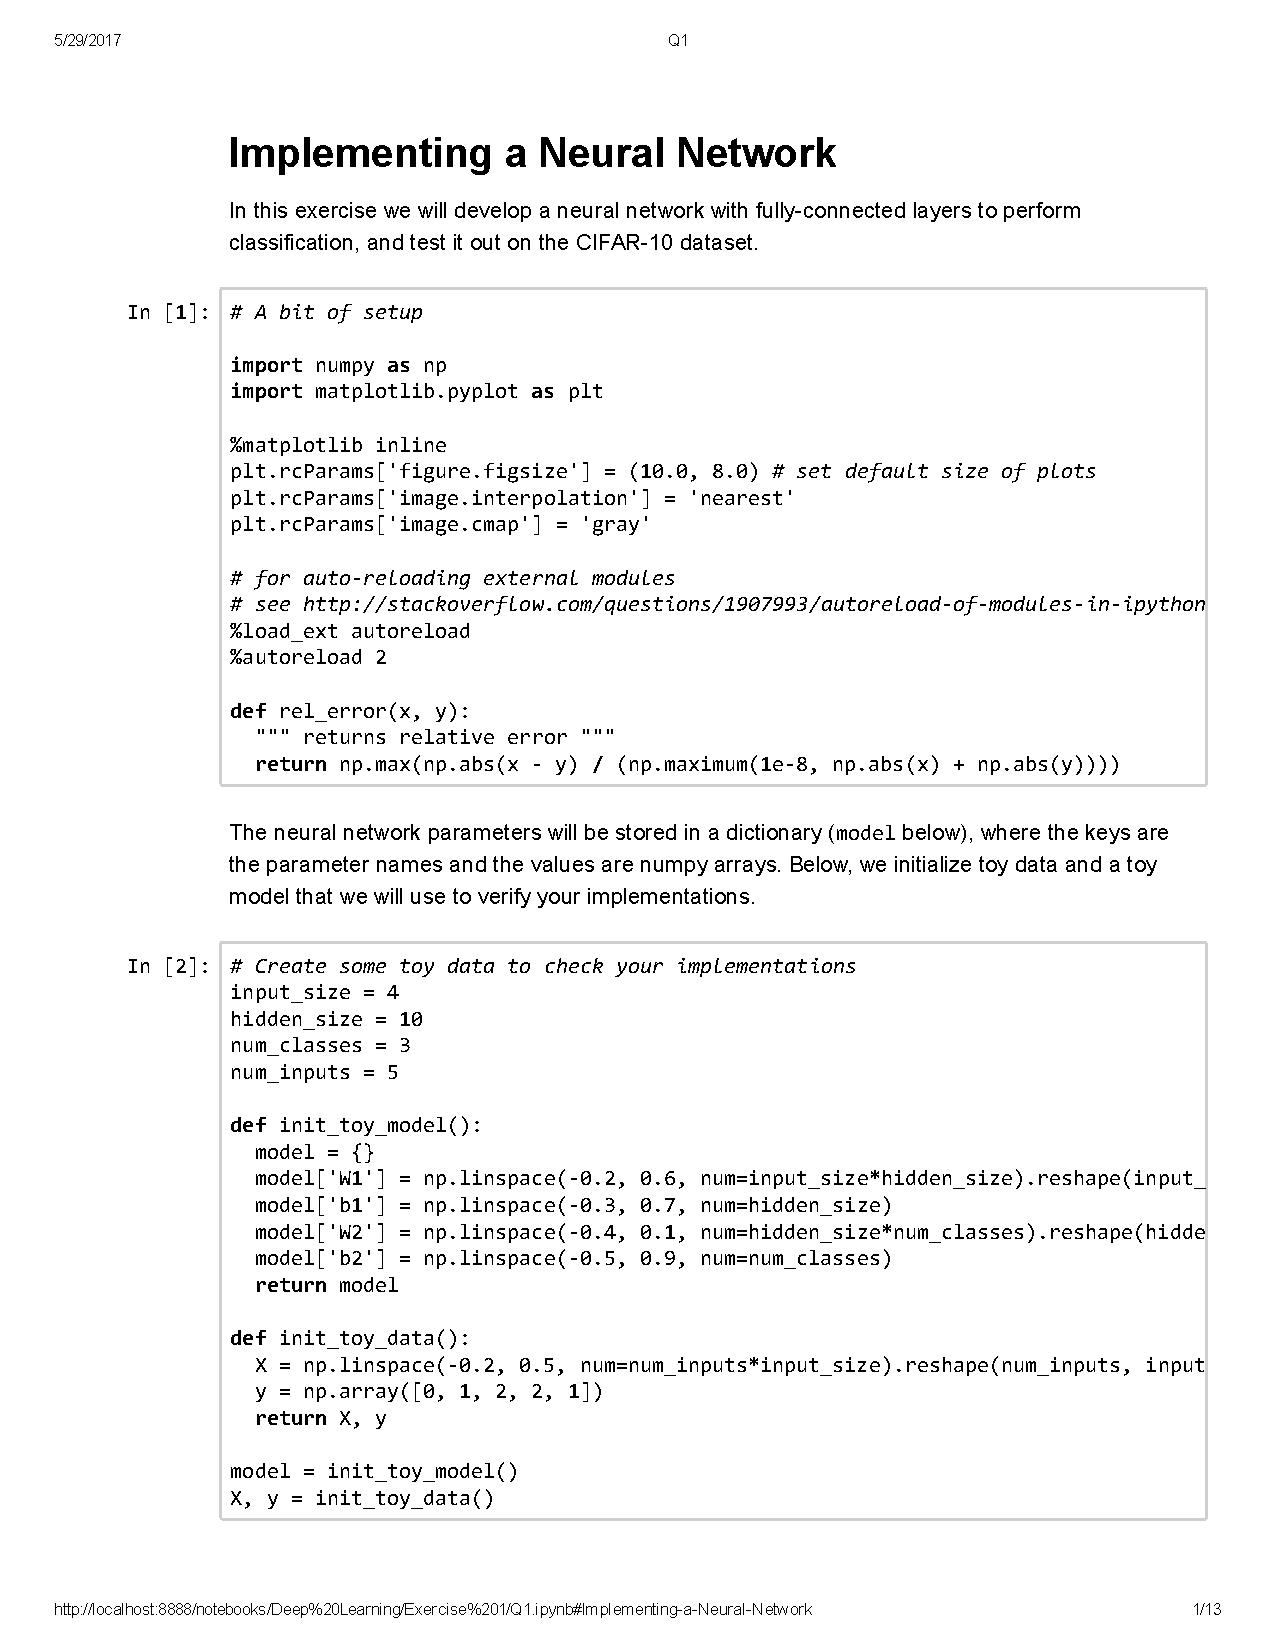
\includepdf[pages=-]{../chapter/appendix/Exercise1/Q1}
\section{Q2}
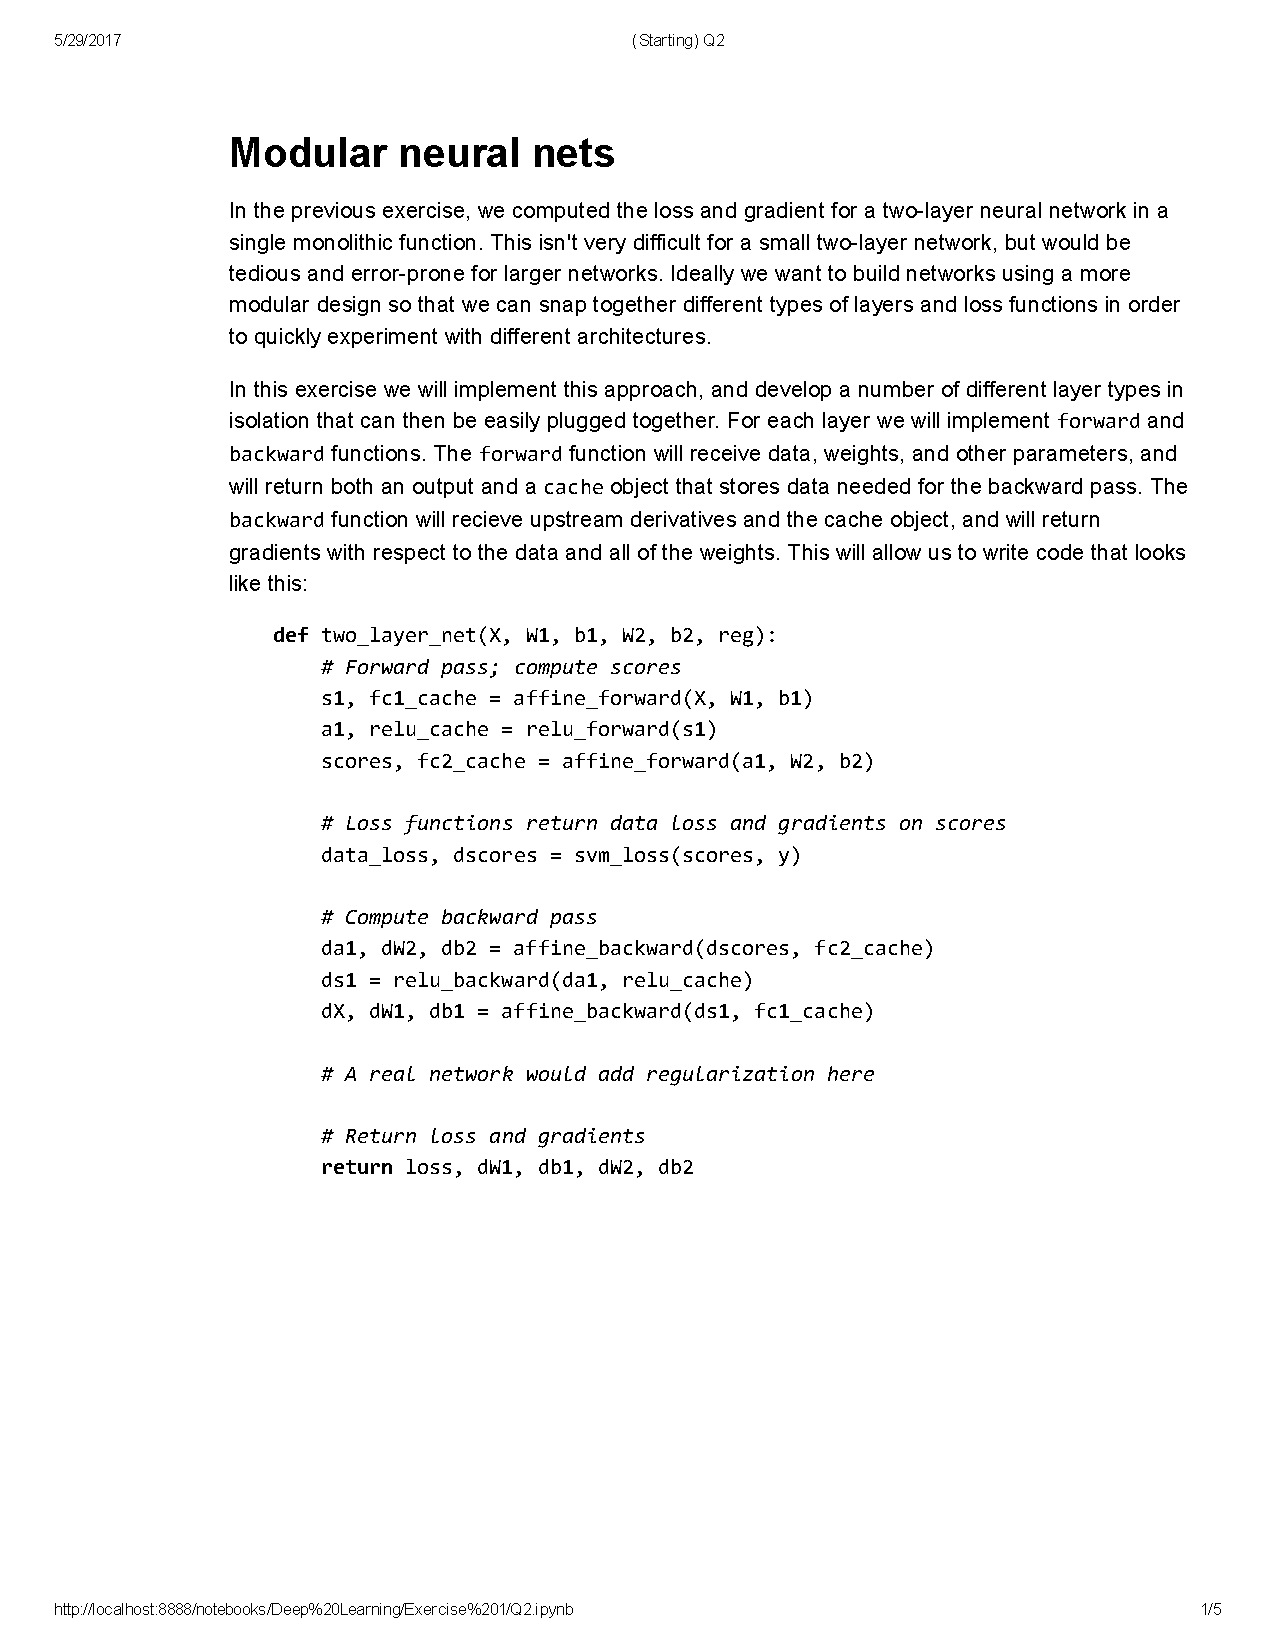
\includepdf[pages=-]{../chapter/appendix/Exercise1/Q2}
\section{Code}
\subsection{neural\_net.py}
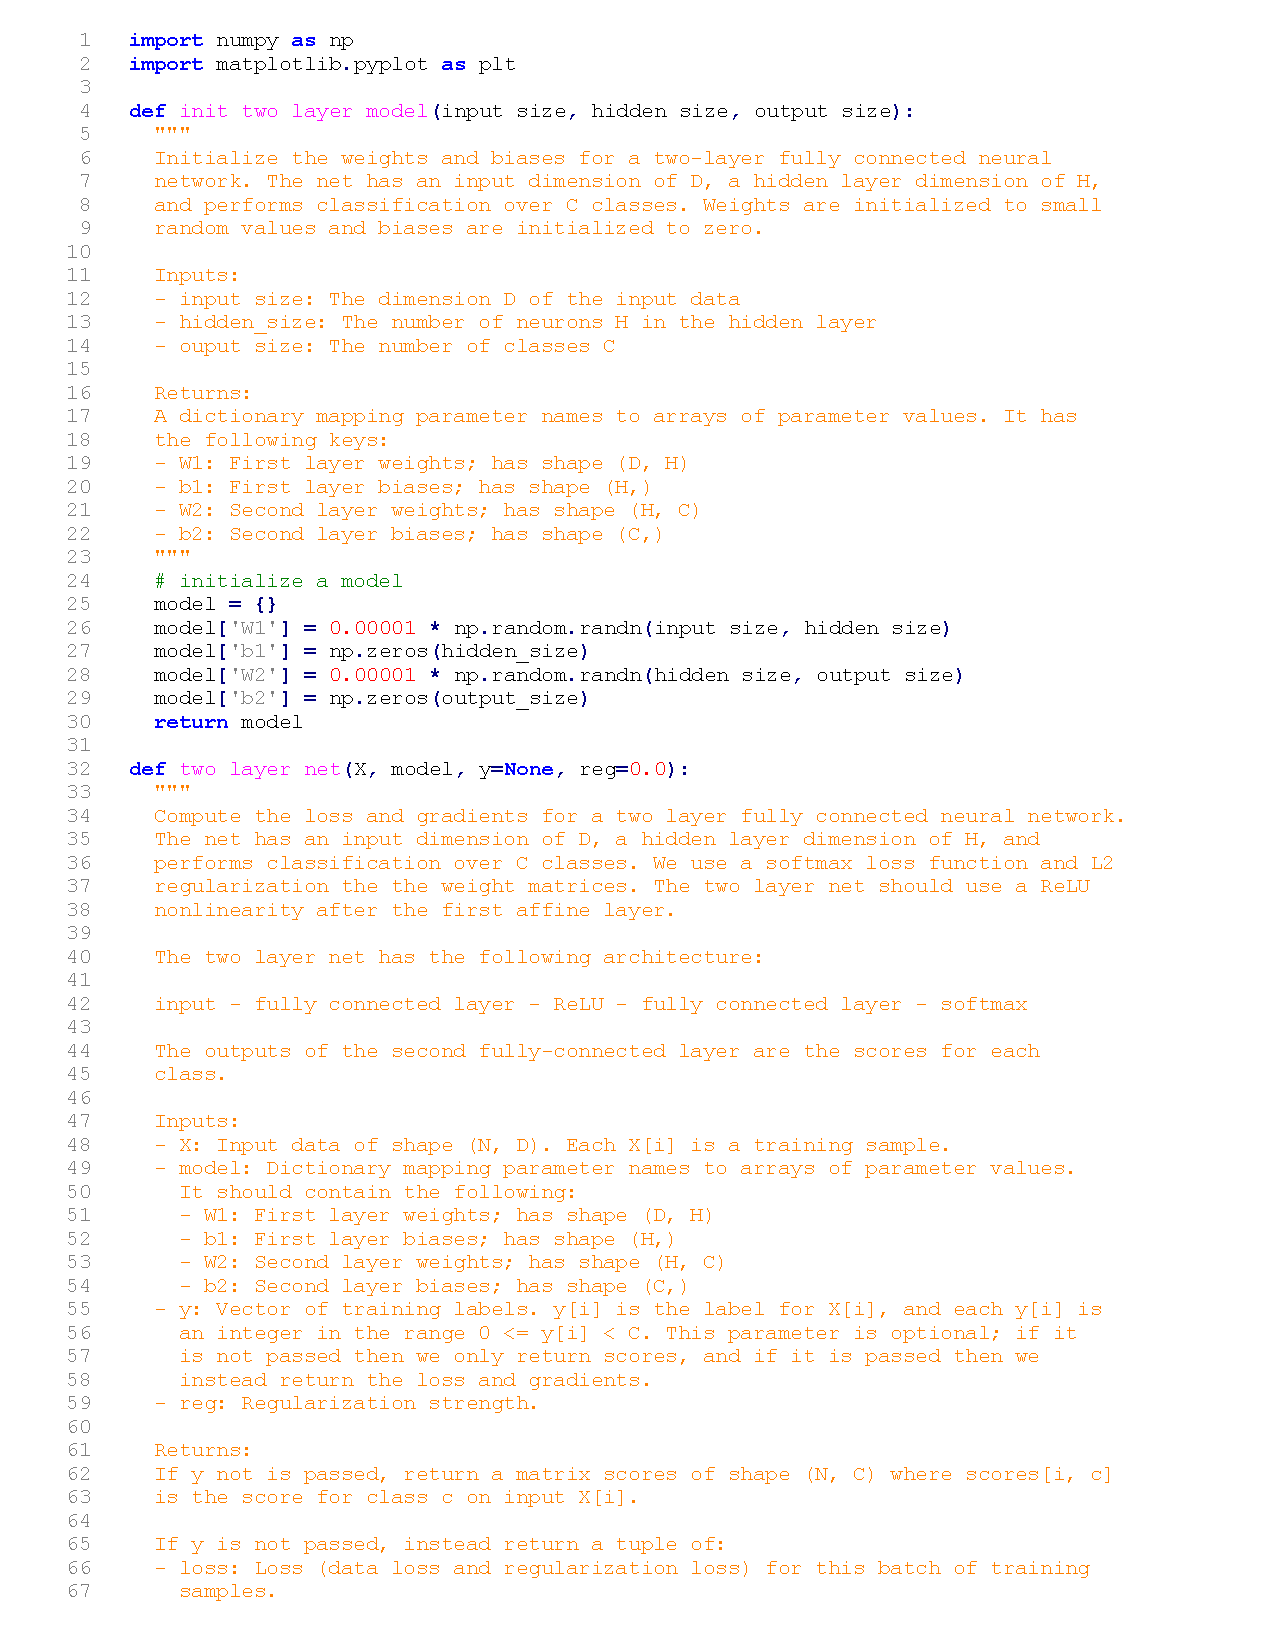
\includepdf[pages=-]{../chapter/appendix/Exercise1/neural_net}
\subsection{layers.py}
\includepdf[pages=-]{../chapter/appendix/Exercise1/layers}
\end{appendices}

\begin{appendices}
\chapter{Exercise 2}
\section{Q1}
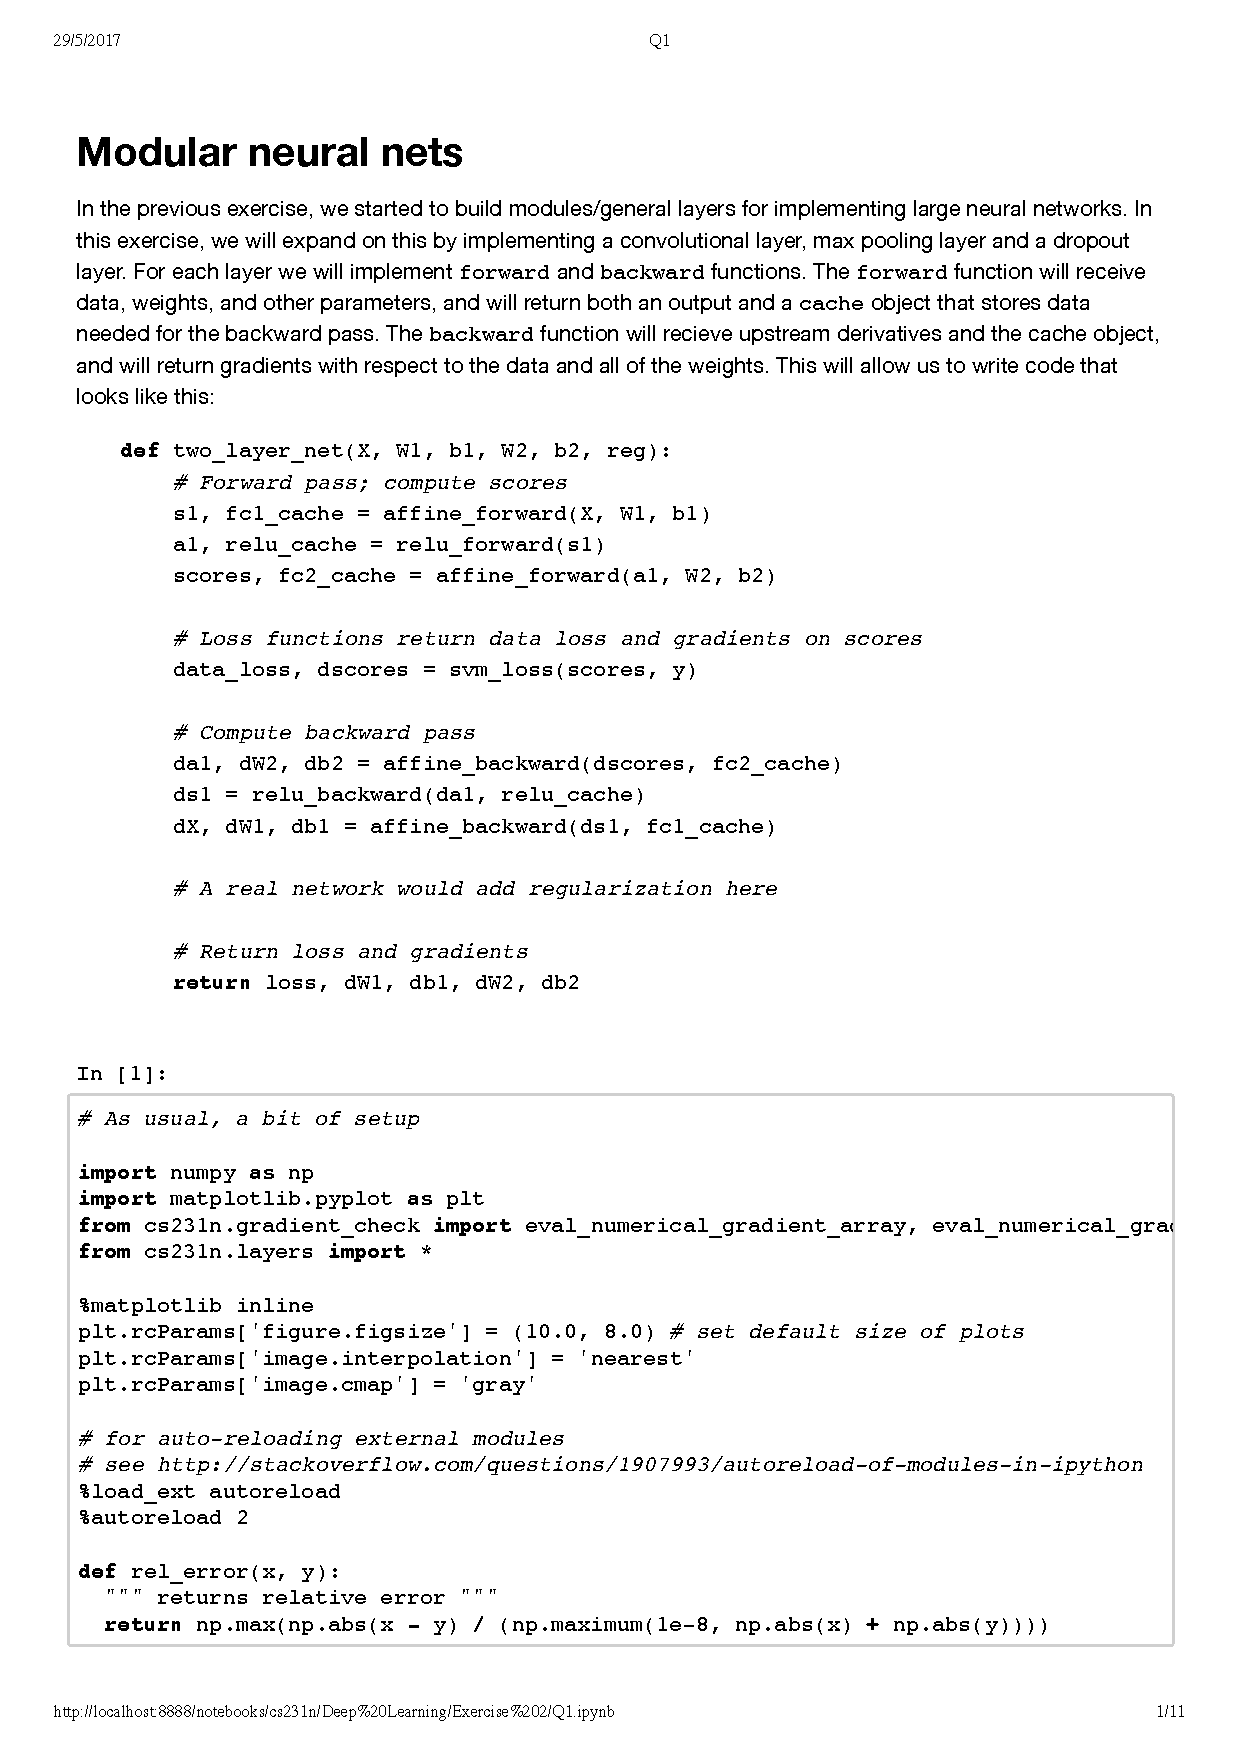
\includepdf[pages=-]{../chapter/appendix/Exercise2/Q1}
\section{Q2}
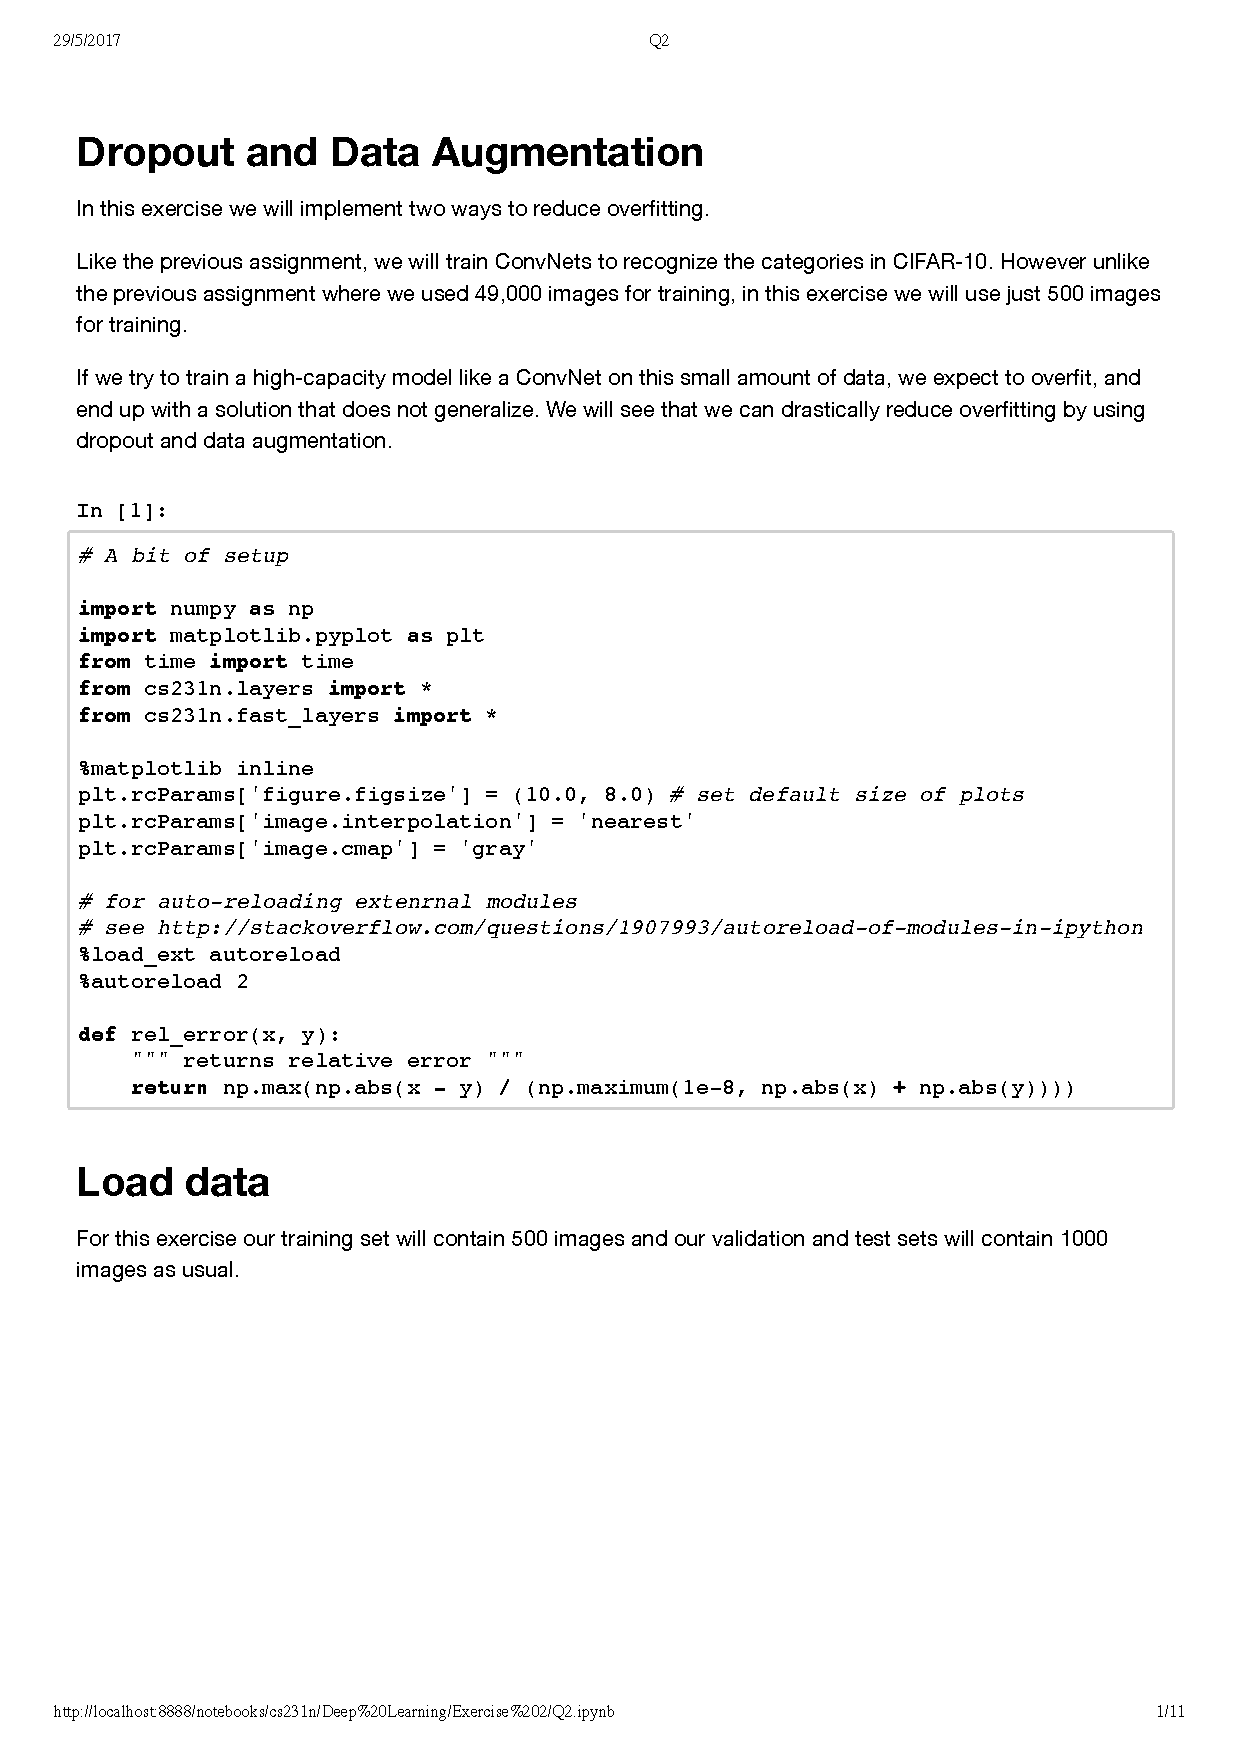
\includepdf[pages=-]{../chapter/appendix/Exercise2/Q2}
\section{Code}
\subsection{layers.py}
\includepdf[pages=-]{../chapter/appendix/Exercise2/layers}
\subsection{data\_augmentation.py}
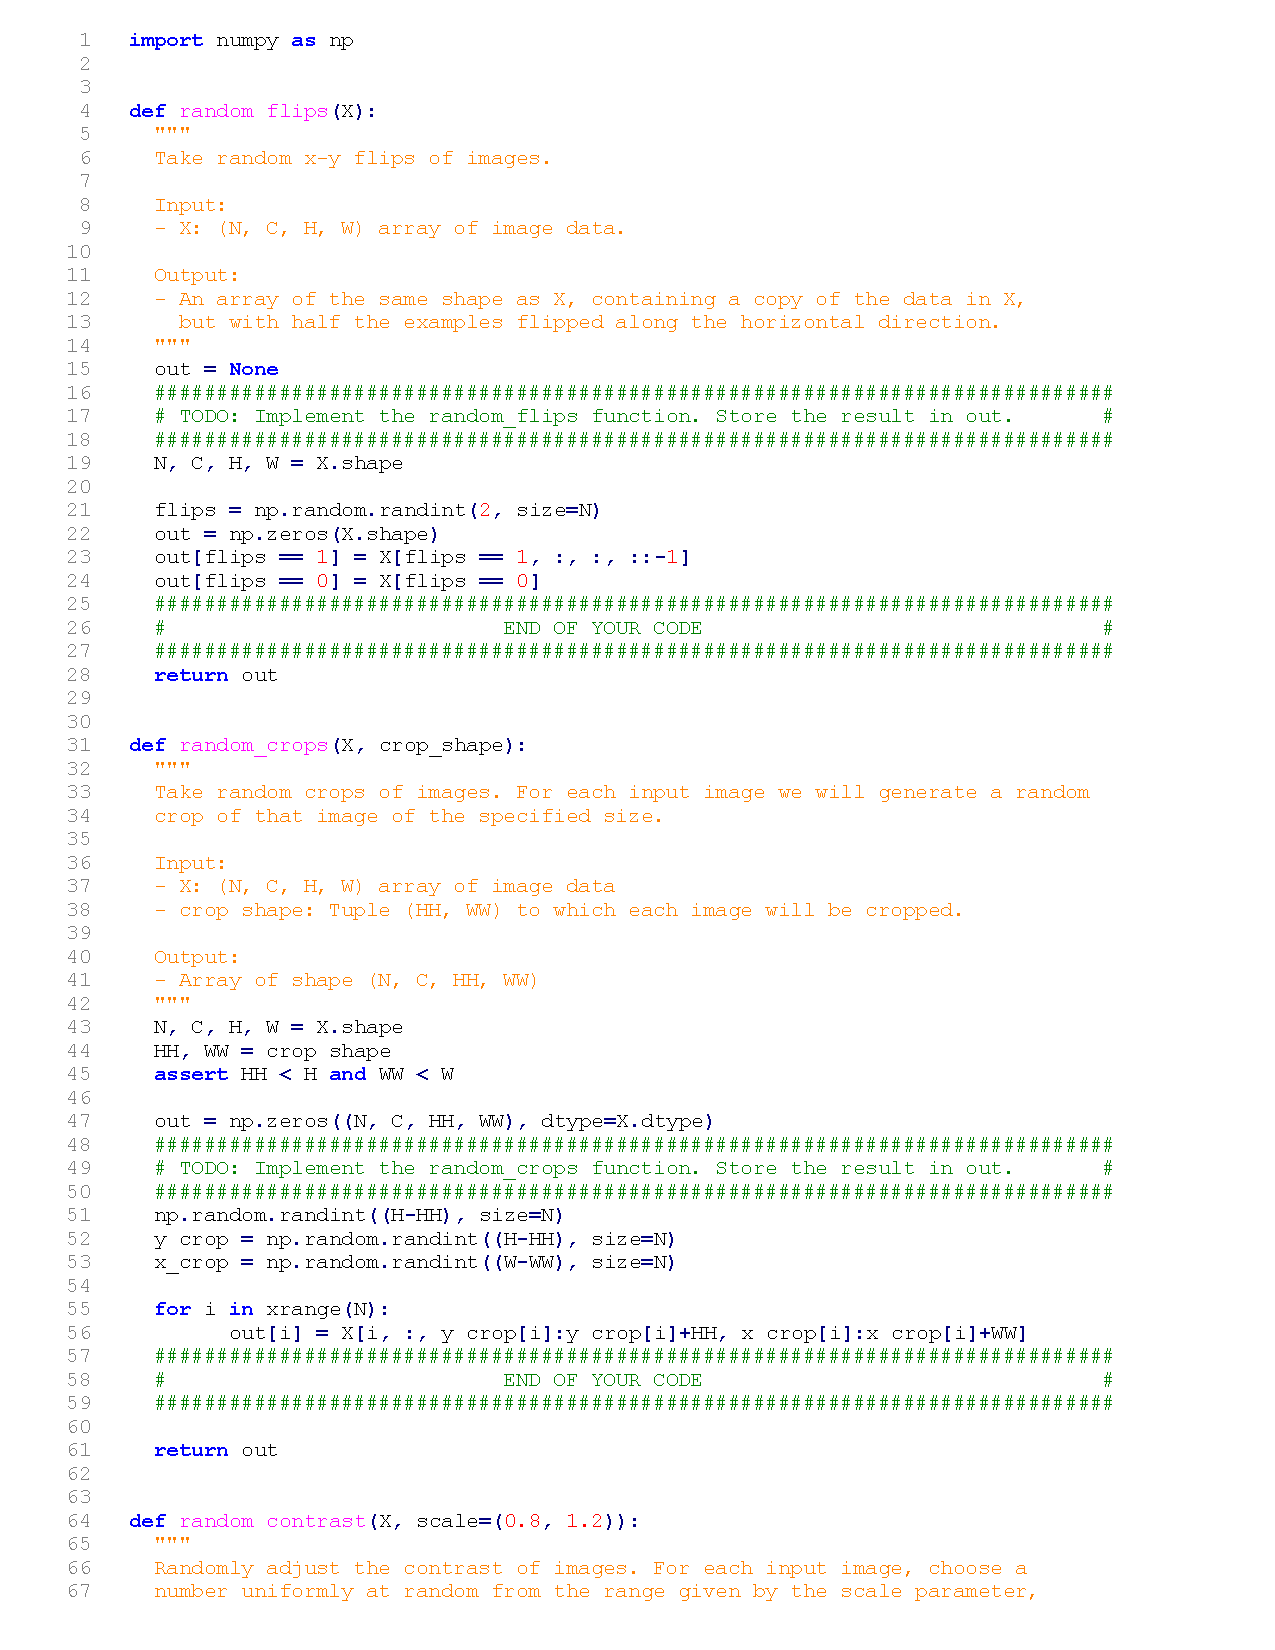
\includepdf[pages=-]{../chapter/appendix/Exercise2/data_augmentation}
\end{appendices}


	\addtocontents{toc}{\protect\setcounter{tocdepth}1}
    
    % Appendix
    \appendix


% Adding appendix to toc and setting space between "Bilag A" and "chapter name"
\addtocontents{toc}{\setlength\cftchapternumwidth{1cm}}

% Redifining chapterstyle for appendix(document past this point)
\chapterstyle{default}
% Changing vertical position of chapter headline
\renewcommand*{\chapterheadstart}{\vspace*{-20pt}}

% Section numbers in margin
%\defaultsecnum
\hangsecnum

% Color setup for sections
% Title color
\renewcommand\thesection{\thechapter.\arabic{section}}

% Set the depth of sections included in table of contents
\settocdepth{chapter} % Changes chapter and section style and toc adding
    

\end{document}
